\part{Metodologia}

\chapter[Metodologia]{Metodologia}

Este capítulo trata da definição do processo de desenvolvimento de software utilizado no presente trabalho, além de um detalhamento acerca de suas atividades e práticas.

\section{Definição do Processo}

O processo de desenvolvimento de software foi construído com base nas práticas e valores do XP, porém com adaptações feitas para um único desenvolvedor. As macro-atividades tentam passar por todas as disciplinas importantes dentro da engenharia de software, além das práticas presentes e cotidianas vindas do XP.

A figura \ref{fig06} representa na forma de fluxograma as macro-atividades definidas neste processo:

\begin{figure}[ht]
	\centering
	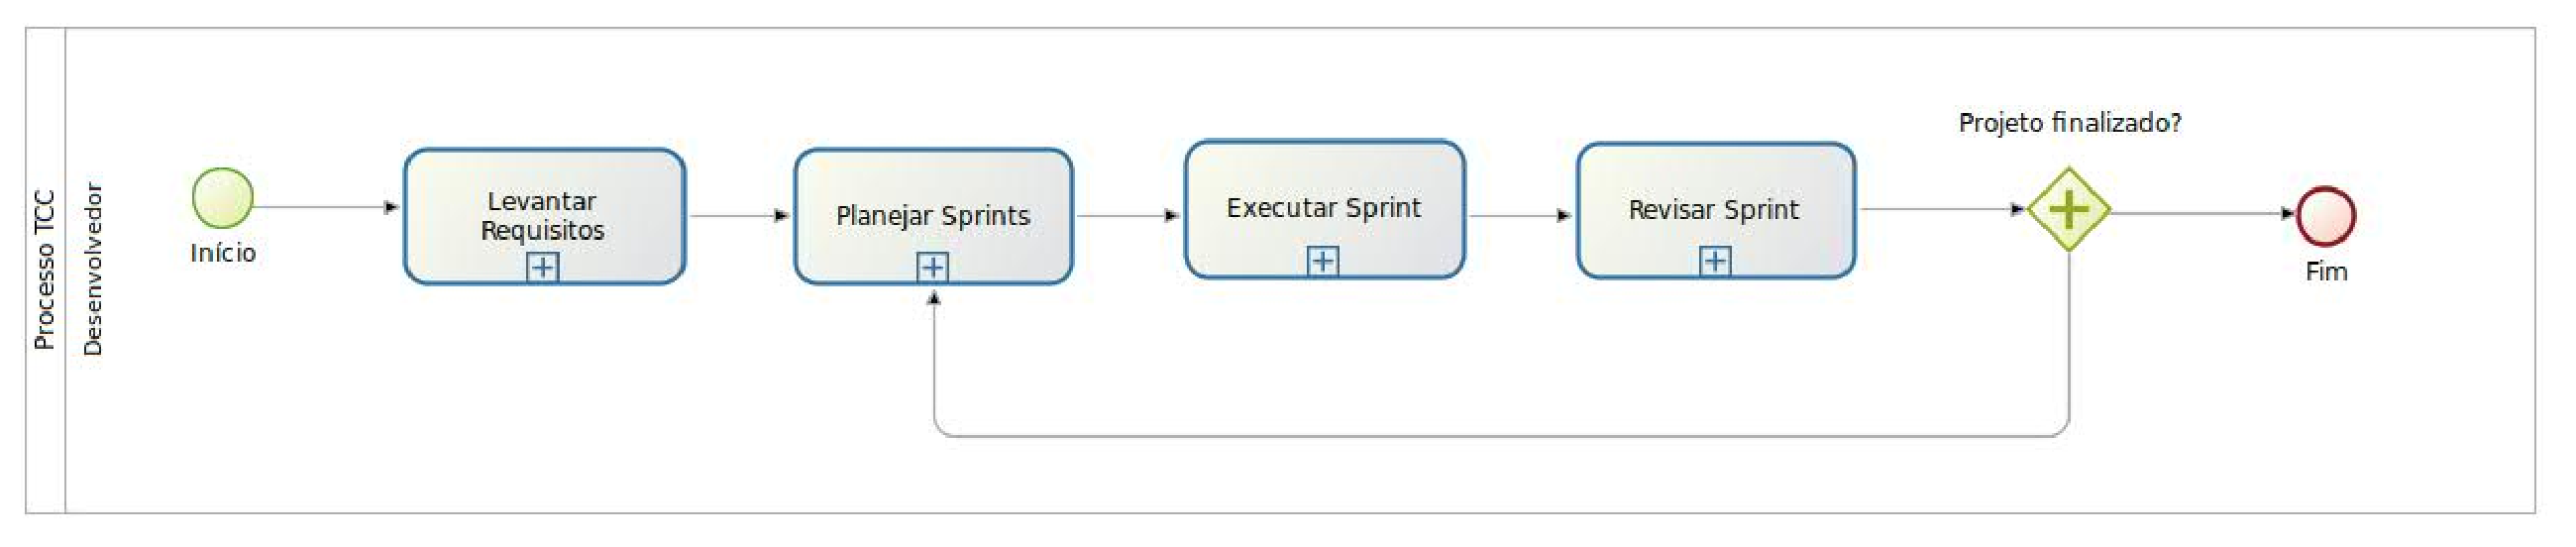
\includegraphics[keepaspectratio=true,scale=0.9, width=\textwidth]{figuras/fig06.eps}
	\caption{Macro-atividades do Processo de Desenvolvimento}
	\label{fig06}
\end{figure}

As macro-atividades tem como propósito o levantamento de requisitos, o desenvolvimento de um produto de qualidade e a entrega contínua de software. As próximas seções farão o detalhamento destas atividades.

\section{Levantar Requisitos}

Esta macro-atividade tem como propósito o entendimento das necessidades dos envolvidos no projeto, o levantamento das features a serem desenvolvidas e a criação de um backlog do produto com as features levantadas. A figura \ref{fig07} representa as atividades do processo e seu fluxo.

\begin{figure}[ht]
	\centering
	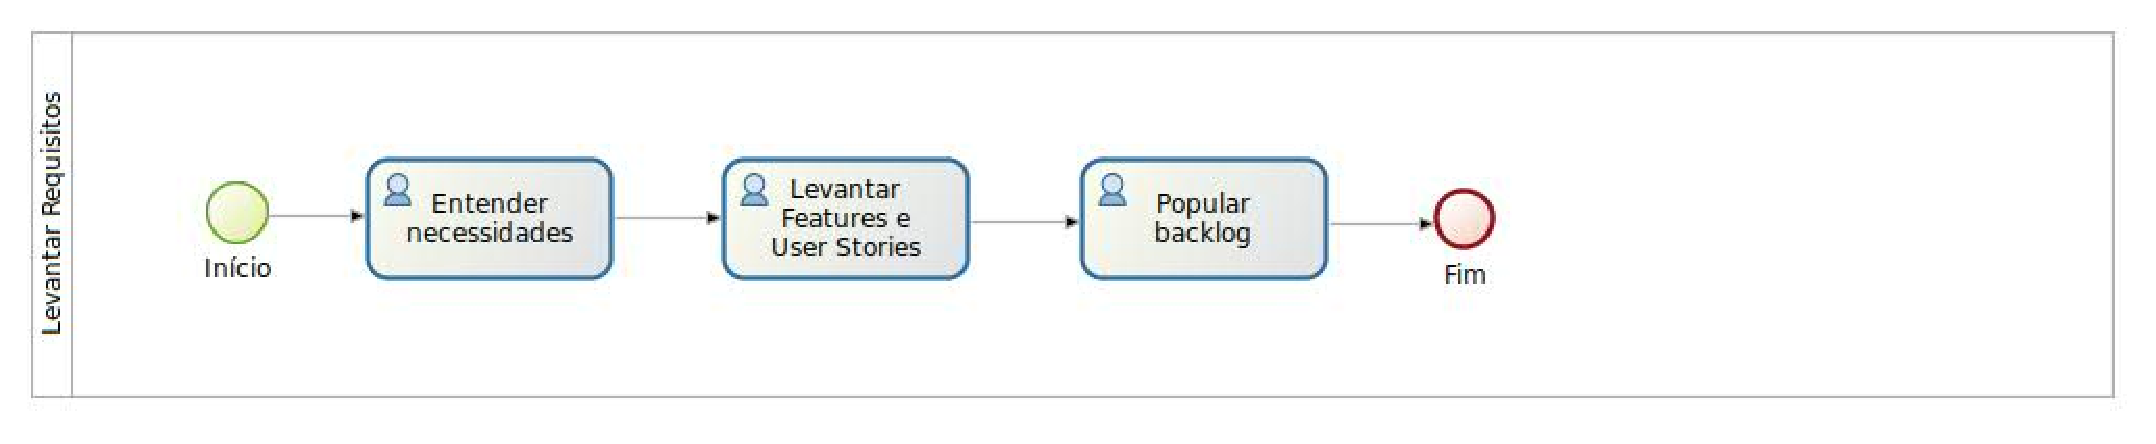
\includegraphics[keepaspectratio=true,scale=0.9, width=\textwidth]{figuras/fig07.eps}
	\caption{Atividade de Levantamento de Requisitos}
	\label{fig07}
\end{figure}

\begin{itemize}

	\item \textbf{Entender Necessidades:} Esta atividade tem o objetivo de entender as necessidades dos envolvidos. Neste caso a STI, como parceira de desenvolvimento, opinará acerca dos requisitos funcionais da aplicação.

	\item \textbf{Levantar Features e User Stories:} Após o levantamento de requisitos, é necessária a definição das \textit{User Stories} e \textit{features}. Ambas estarão definidas e descritas como \textit{issues} no repositório do projeto.

	\item \textbf{Popular Backlog:} Um \textit{backlog} será criado no repositório do projeto, contendo as \textit{User Stories} definidas no levantamento inicial do projeto. Durante o andamento do mesmo, novas \textit{features} poderão ser acrescentadas.

\end{itemize}

\section{Planejar Sprints}

O foco desta atividade é priorizar as \textit{issues} a serem desenvolvidas durante uma \textit{sprint}, ou um ciclo de desenvolvimento em metodologias ágeis,  tendo a duração de 15 dias. Além de adequar o escopo de cada ciclo à capacidade do desenvolvedor.A figura \ref{fig08} representa as atividades do processo e seu fluxo.

\begin{figure}[ht]
	\centering
	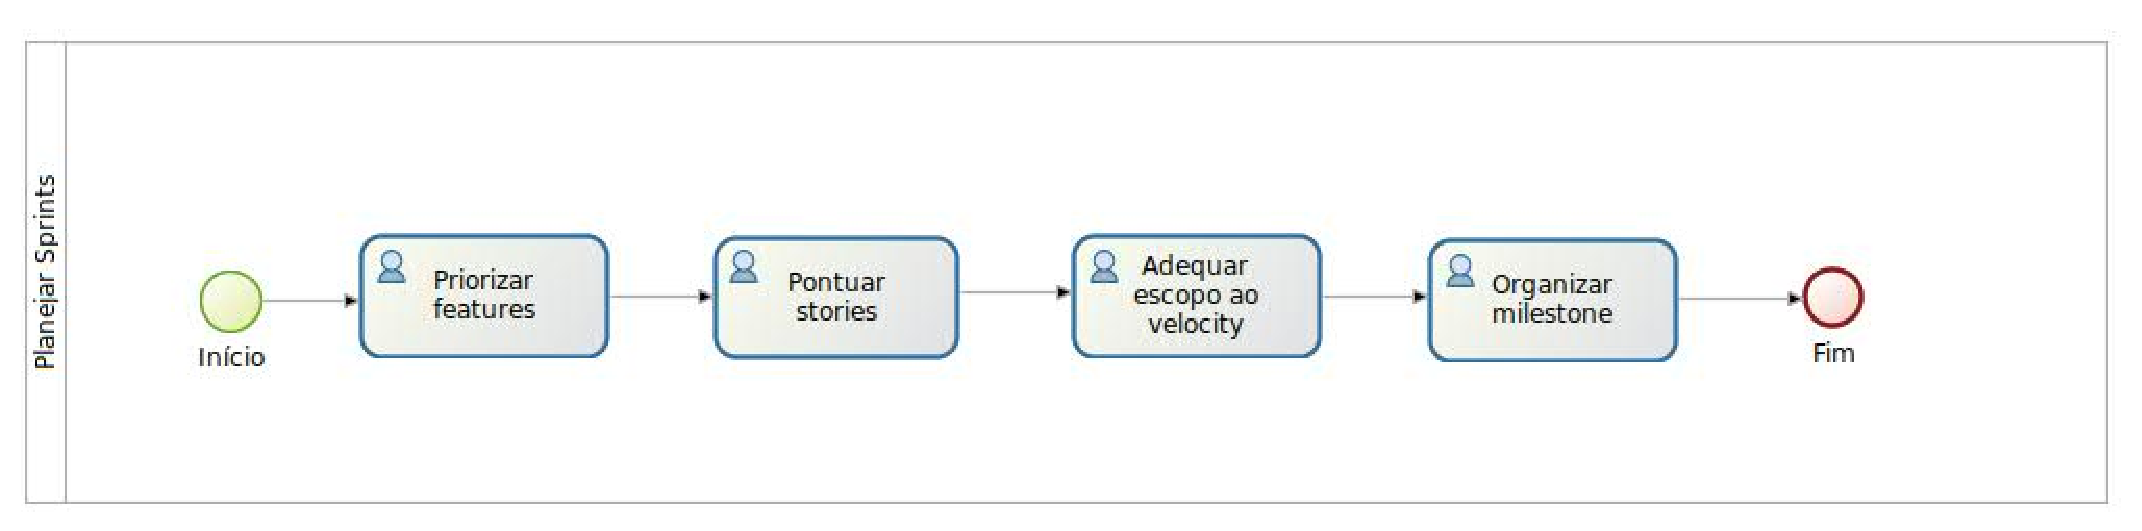
\includegraphics[keepaspectratio=true,scale=0.9, width=\textwidth]{figuras/fig08.eps}
	\caption{Atividade de Planejamento de Sprints}
	\label{fig08}
\end{figure}

\begin{itemize}

	\item \textbf{Priorizar Features:} Esta atividade tem o objetivo de priorizar as \textit{features} mais importantes, ou que trarão maior valor ao cliente dentro do projeto. Esta atividade será feita por meio de reuniões com a STI.

	\item \textbf{Pontuar Stories:} Definir um número que caracteriza a dificuldade do desenvolvimento de uma \textit{user story}. Este número pode ser definido através de experiências dos desenvolvedores ou análise de riscos. É recomendado que essa numeração siga a sequência de Fibonacci.

	\item \textbf{Adquar Escopo ao Velocity:} Esta atividade tem a finalidade de avaliar a pontuação definida na priorização das \textit{issues} a serem desenvolvidas na \textit{sprint}. O desenvolvedor pode ter uma ideia de sua capacidade de produção comparando os valores da \textit{sprint} atual com os anteriores. O número de pontos de uma sprint nunca deve ser muito maior que o da anterior ou da média das anteriores. Chamamos essa média de \textit{velocity}.

	\item \textbf{Organizar Milestone:} Esta atividade se restringe ao repositório do projeto. Nele serão assinaladas as issues priorizadas para aquela sprint, além de uma descrição de sua finalidade e status.

\end{itemize}

\section{Executar Sprint}

Esta macro-atividade tem o objetivo de desenvolver as \textit{features} priorizadas na atividade anterior, utilizando práticas presentes no XP, como integração contínua, testes automatizados e \textit{deploy} de pequenos incrementos de software ao final de cada ciclo de desenvolvimento. A figura \ref{fig09} representa em forma de fluxograma as atividades do processo.

\begin{figure}[ht]
	\centering
	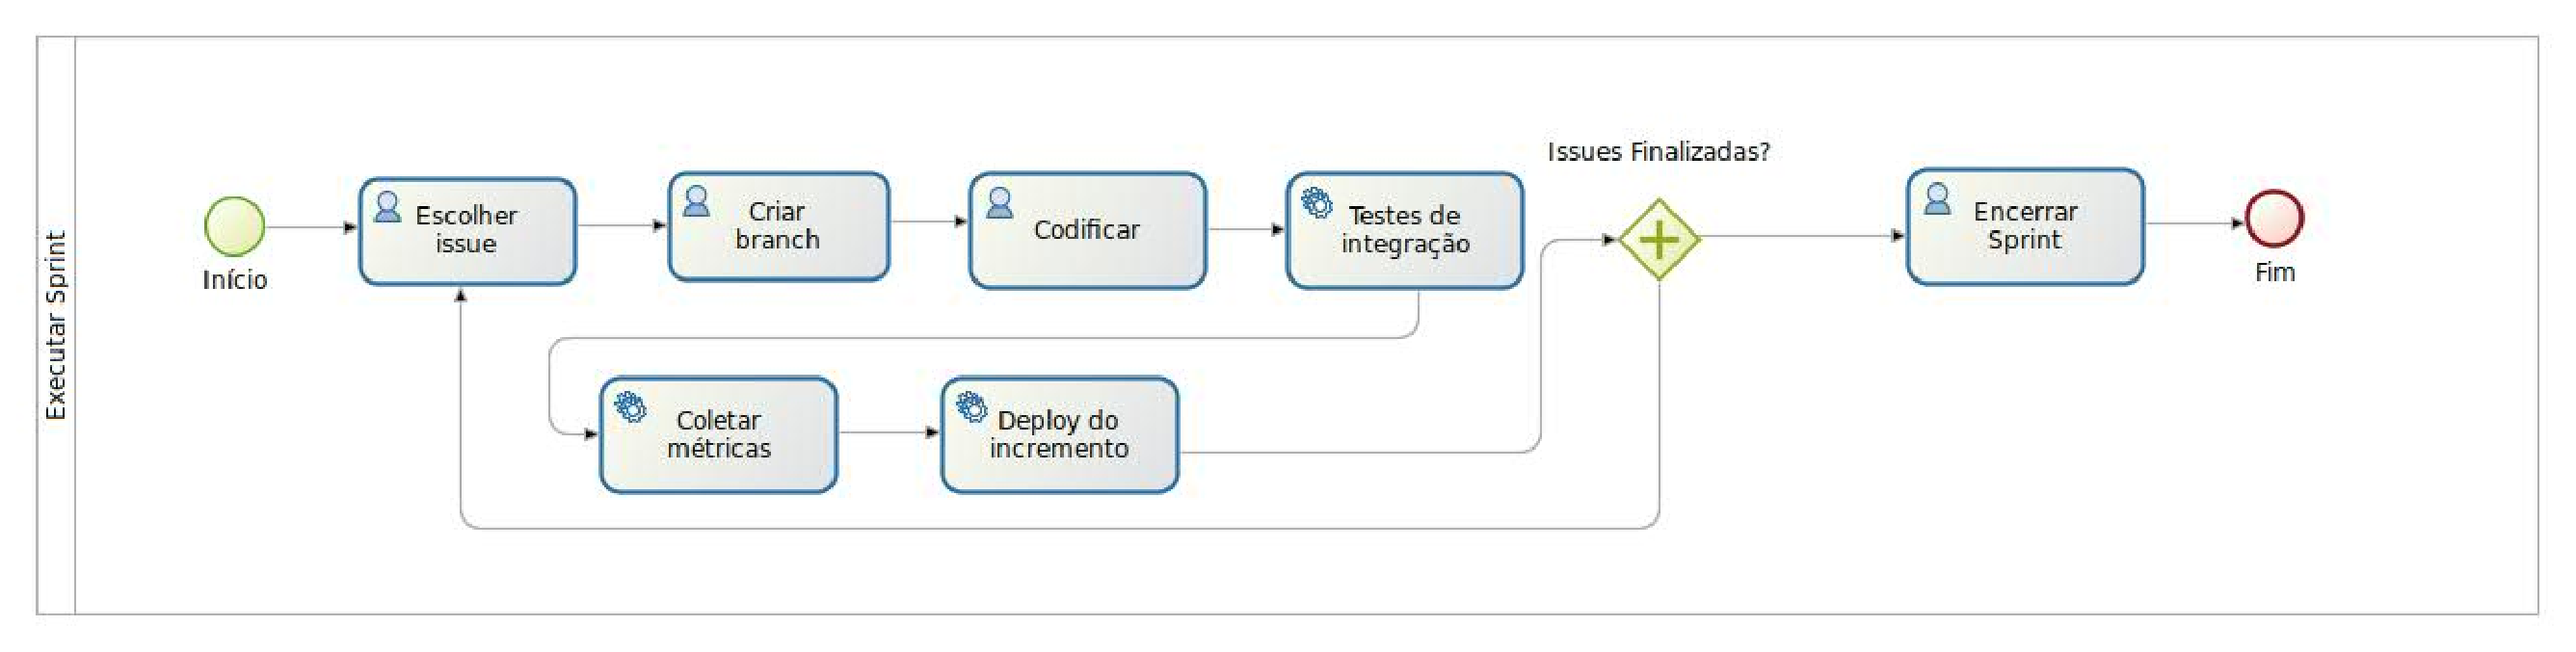
\includegraphics[keepaspectratio=true,scale=0.9, width=\textwidth]{figuras/fig09.eps}
	\caption{Atividade de Execução da Sprint}
	\label{fig09}
\end{figure}

\begin{itemize}

	\item \textbf{Escolher issue:} Definir uma \textit{issue} a ser desenvolvida durante a sprint.

	\item \textbf{Criar Branch:} Cria uma nova \textit{branch} para o desenvolvimento da \textit{issue}. Ao final do desenvolvimento da mesma, essa \textit{branch} será integrada a \textit{branch} principal do projeto (Master).

	\item \textbf{Codificar:} Atividade padrão de codificação, onde práticas como testes unitários, refatoração, código simples e padrões de código serão aplicadas.

	\item \textbf{Testes de Integração:} Testes automatizados feitos por ferramentas. Testes como esse impedem a integração de \textit{commits} a uma \textit{branch} caso existam testes quebrados, ou a qualidade do código diminua.

	\item \textbf{Coletar Métricas:} Ferramentas de análise estática de código  irão coletar métricas a fim de orientar o desenvolvedor acerca da qualidade de código.

	\item \textbf{Deploy de Incremento:} Após o término do desenvolvimento da \textit{issue}, a \textit{branch} será integrada a master e uma nova versão do produto será disponibilizada no servidor de produção.

\end{itemize}

Com a \textit{issue} finalizada, caso existam outras definidas para a \textit{sprint}, o desenvolvedor repetirá o processo até que todas sejam finalizadas. A última atividade do processo encerra a \textit{sprint}, fechando todas as \textit{issues} no repositório.

\section{Revisar Sprint}

Esta atividade tem como objetivo revisar métricas de código a fim de que refatorações possam ocorrer nos próximos ciclos de desenvolvimento. Também tem como objetivo separar \textit{issues} não finalizadas para que sejam realocadas na próxima \textit{sprint}. A figura \ref{fig10} representa em forma de fluxograma as atividades do processo.

\begin{figure}[ht]
	\centering
	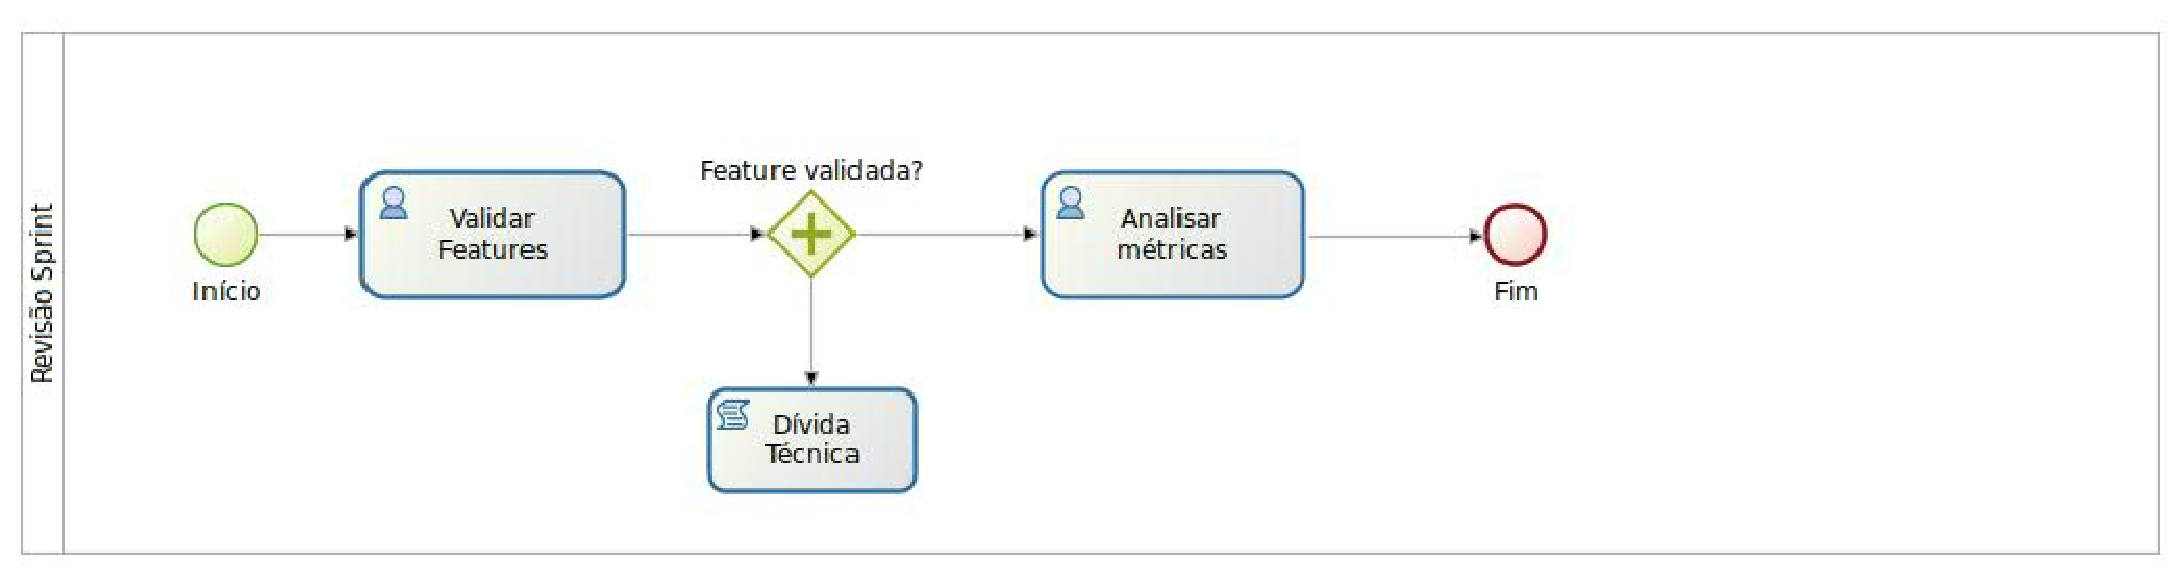
\includegraphics[keepaspectratio=true,scale=0.9, width=\textwidth]{figuras/fig10.eps}
	\caption{Atividade de Revisão da Sprint}
	\label{fig10}
\end{figure}

\begin{itemize}

	\item \textbf{Validar Features:} Nesta atividade o desenvolvedor valida as \textit{features} desenvolvidas durante a \textit{sprint}. Esta validação pode ser feita através de testes de aceitação ou feita pela STI por comentários nas \textit{issues} do repositório.

	\item \textbf{Analisar Métricas:} Ao fazer uma análise das métricas é possível aferir a qualidade do código e definir pontos para refatoração na \textit{sprint} seguinte.

	\item \textbf{Dívida Técnica:} Caso as \textit{features} não sejam validadas ou não tiverem sido concluídas durante a \textit{sprint}, são consideradas dívidas técnicas e separadas para serem novamente desenvolvidas na próxima \textit{sprint}.

\end{itemize}

Este capítulo dissertou sobre a metodologia definida para o desenvolvimento do presente trabalho, além de detalhar suas atividades. O próximo capítulo fará um relato dos resultados obtidos até o momento.
